\documentclass[11pt]{beamer}
\usepackage[utf8]{inputenc}
\usepackage{graphicx, epsfig}
\usepackage{amsmath,mathrsfs,amsfonts,amssymb}
%\usepackage{subfig}
\usepackage{floatflt}
\usepackage{epic,ecltree}
\usepackage{mathtext}
\usepackage{fancybox}
\usepackage{fancyhdr}
\usepackage{multirow}
\usepackage{enumerate}
\usepackage{epstopdf}
\usepackage{multicol}
\usepackage{algorithm}
\usepackage[noend]{algorithmic}
\usepackage{tikz}
\usepackage{blindtext}
\usetheme{default}%{default}%{Singapore}%{Warsaw}%{Warsaw}%{Darmstadt}
\usecolortheme{default}
\setbeamerfont{title}{size=\Huge}
\setbeamertemplate{footline}[page number]{}


\makeatletter
\newcommand\HUGE{\@setfontsize\Huge{35}{40}}
\makeatother    

\setbeamerfont{title}{size=\HUGE}
\beamertemplatenavigationsymbolsempty

% latin bold lower
\newcommand{\ba}{\mathbf{a}} 
\newcommand{\bc}{\mathbf{c}} 
\newcommand{\be}{\mathbf{e}} 
\newcommand{\bh}{\mathbf{h}} 
\newcommand{\bp}{\mathbf{p}} 
\newcommand{\bt}{\mathbf{t}} 
\newcommand{\bs}{\mathbf{s}} 
\newcommand{\bu}{\mathbf{u}} 
\newcommand{\bv}{\mathbf{v}} 
\newcommand{\bw}{\mathbf{w}} 
\newcommand{\bx}{\mathbf{x}} 
\newcommand{\by}{\mathbf{y}} 
\newcommand{\bz}{\mathbf{z}} 

% latin bold upper
\newcommand{\bA}{\mathbf{A}} 
\newcommand{\bB}{\mathbf{B}} 
\newcommand{\bC}{\mathbf{C}} 
\newcommand{\bI}{\mathbf{I}} 
\newcommand{\bL}{\mathbf{L}} 
\newcommand{\bM}{\mathbf{M}} 
\newcommand{\bQ}{\mathbf{Q}} 
\newcommand{\bT}{\mathbf{T}} 
\newcommand{\bU}{\mathbf{U}} 
\newcommand{\bV}{\mathbf{V}} 
\newcommand{\bW}{\mathbf{W}} 
\newcommand{\bX}{\mathbf{X}} 
\newcommand{\bY}{\mathbf{Y}} 
\newcommand{\bZ}{\mathbf{Z}} 

% latin cal upper
\newcommand{\cG}{\mathcal{G}} 
\newcommand{\cL}{\mathcal{L}} 
\newcommand{\cN}{\mathcal{N}} 
\newcommand{\cS}{\mathcal{S}} 
\newcommand{\cT}{\mathcal{T}} 
\newcommand{\cW}{\mathcal{W}} 
\newcommand{\cX}{\mathcal{X}} 
\newcommand{\cZ}{\mathcal{Z}} 

% latin bb upper
\newcommand{\bbE}{\mathbb{E}} 
\newcommand{\bbI}{\mathbb{I}} 
\newcommand{\bbP}{\mathbb{P}} 
\newcommand{\bbR}{\mathbb{R}} 

% greek bold lower
\newcommand{\bepsilon}{\boldsymbol{\epsilon}} 
\newcommand{\btheta}{\boldsymbol{\theta}} 
\newcommand{\blambda}{\boldsymbol{\lambda}} 
\newcommand{\bpi}{\boldsymbol{\pi}} 
\newcommand{\bmu}{\boldsymbol{\mu}} 
\newcommand{\bsigma}{\boldsymbol{\sigma}} 
\newcommand{\bphi}{\boldsymbol{\phi}} 

% greek bold upper
\newcommand{\bSigma}{\boldsymbol{\Sigma}} 

\DeclareMathOperator*{\argmin}{arg\,min}
\DeclareMathOperator*{\argmax}{arg\,max}
\newcommand{\createdgmtitle}[1]{\title[\hbox to 56mm{Mathematical Forecasting Methods \hfill\insertframenumber\,/\,\inserttotalframenumber}]
	{\vspace{1.5\cm} \\ Mathematical Forecasting Methods \\ {\Huge Лекция #1}}
	\author{}
	\institute{
	МФТИ
	} 
	\date{Осень, 2023}
}

\newcommand\myfootnote[1]{%
  \tikz[remember picture,overlay]
  \draw (current page.south west) +(1in + \oddsidemargin,0.5em)
  node[anchor=south west,inner sep=0pt]{\parbox{\textwidth}{%
      \rlap{\rule{10em}{0.4pt}}\raggedright\scriptsize \textit{#1}}};}

\newcommand\myfootnotewithlink[2]{%
  \tikz[remember picture,overlay]
  \draw (current page.south west) +(1in + \oddsidemargin,0.5em)
  node[anchor=south west,inner sep=0pt]{\parbox{\textwidth}{%
      \rlap{\rule{10em}{0.4pt}}\raggedright\scriptsize\href{#1}{\textit{#2}}}};}
\createdgmtitle{3}
\usepackage{tikz}
\usepackage{amsmath}
\usepackage[english,russian]{babel}
\usepackage[labelformat=empty]{caption}

\usepackage{csquotes}

\usetikzlibrary{arrows,shapes,positioning,shadows,trees}
\newcommand*{\defeq}{\stackrel{\text{def}}{=}}

%--------------------------------------------------------------------------------
\begin{document}
%--------------------------------------------------------------------------------
\begin{frame}[noframenumbering,plain]
%\thispagestyle{empty}
\titlepage
\end{frame}
%=======
\begin{frame}{Краткое повторение}
\begin{itemize}
\item \textbf{Временной ряд} --- это совокупность значения параметра $\{x_1, x_2,...,x_T\}= \{ x_t \}_{t=1}^T$, изменяющегося во времени,  через равные промежутки времени.
\item \textbf{Также рассматриваем как:} совокупность случайных величин (\textit{дискретный случайный или стохастический процесс}), где для каждого \textit{t} значение рассматривается как случайная величина.
\item \textbf{Задача прогнозирования}: найти функции $f_{T,d}$:
\begin{equation*}
x_{T+d} \approx f_{T,d}(x_1,...x_T;w) =: \hat{x}_{T+d}, 
\end {equation*}
где $f_{T,d}$ --- модель временного ряда, $d =1,...,D$ --- горизонт прогнозирования.
\end{itemize}

\end{frame}
%=======
\begin{frame}{Краткое повторение}
\textbf{Определение.} Временной ряд $\{x_i\}_{i=1}^{T}$ называется слабо стационарным (или стационарным в широком смысле), если
\begin{itemize}
    \item $\mathrm{E}[x_t]=$ const (т.е. временной ряд не имеет \textit{тренда}),
    \item $\mathrm{Cov}(x_t,x_{t+k}) = \mathrm{E}[(x_t - \mathrm{E}x_t)(x_{t+k} - \mathrm{E}x_{t+k})] = \gamma(k)$ (ковариация зависит только от разницы во времени).
\end{itemize}
\begin{figure}
    \centering
    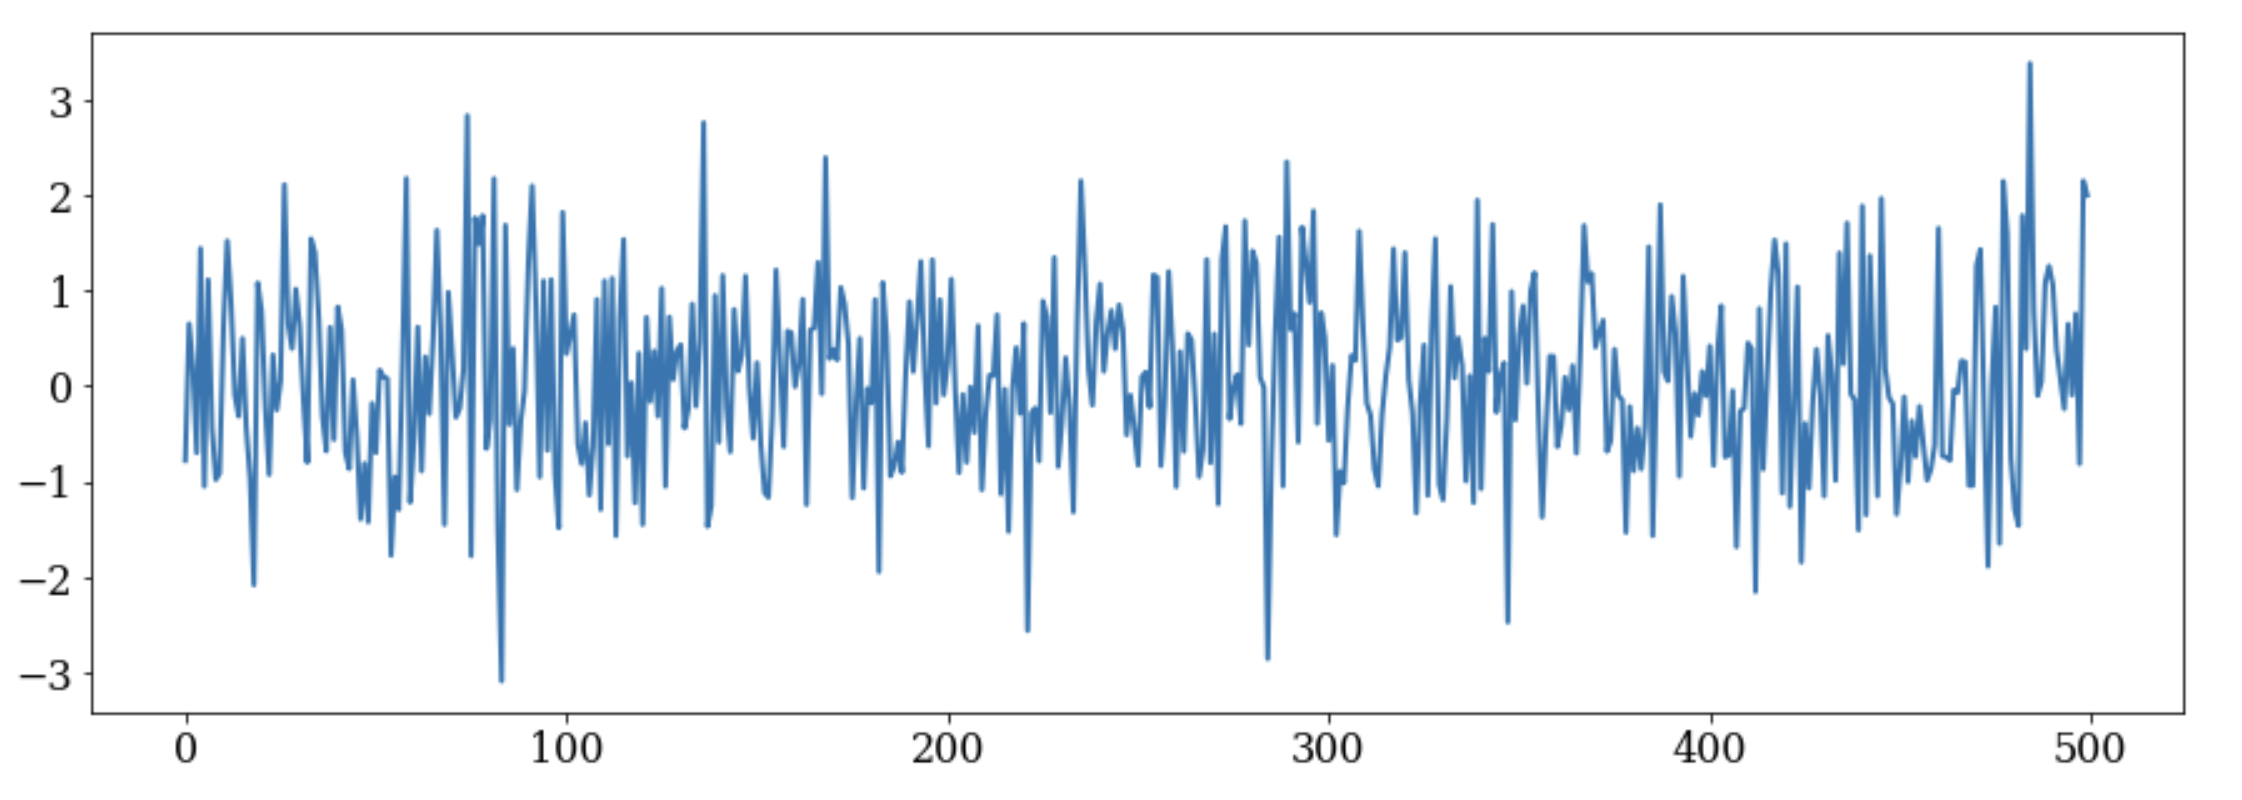
\includegraphics[width=0.9\linewidth]{lecture_3/fig/noise.png}
    \caption{Белый шум}
\end{figure}
\end{frame}
%=======
\begin{frame}{Краткое повторение}
\textbf{Модель SARIMAX($p, q, d; P, Q, D$)} приводит временной ряд к стационарному виду и прогнозирует с наперед заданной точностью (по Теореме Вольда).
\begin{equation*}
    \begin{aligned}
    x_t = \mu &
    + \underbrace{\phi_1 x_{t-1} + \phi_2 x_{t-2} + ...}_{p\text{ слагаемых AR}}
    + \underbrace{u_t + \theta_1 u_{t-1} + \theta_2 u_{t-2} + ...}_{q\text{ слагаемых MA}}\\
    &+ \underbrace{\alpha_1 x_{t-S} + \alpha_2 x_{t-2S}+ ...}_{P\text{ сезонных слагаемых AR}}
    + \underbrace{\eta_1 u_{t-S} + \eta_2 u_{t-2S}+ ...}_{Q\text{ сезонных слагаемых MA}}\\
    &+ \underbrace{\beta_1 z_1 + \beta_2 z_2 + \beta_3 z_3+ ...}_{\text{внешние переменные, не зависящие от } x_t},
    \end{aligned}
\end{equation*}
где $\phi, \theta, \alpha, \eta, \beta$ --- настраиваемые параметры модели,\\
$x_t$ --- значения временного ряда (продифференцированные d и D сезонных раз),\\
$u_t$ --- значения шумов,\\
$z_i$ --- внешние (экзогенные) переменные.
\end{frame}
%=======
\begin{frame}{Подбор параметров модели}
\begin{itemize}
    \item Если все гиперпараметры модели $p, q, d; P, Q, D$ подобраны, то коэффициенты авторегрессии подбираются методом МНК;
    \item Для выбора $\theta$ шумовая компонента предварительно оценивается на остатках \textquote{простой} авторегрессии;
    \item Если шум гауссовский, то МНК дает оценки максимального правдоподобия.
\end{itemize}
\textbf{Вопрос:} как подбирать приближение для $p, q, d; P, Q, D$?
\end{frame}
%=======
\begin{frame}{Информационные критерии}

\textbf{Критерий Акаике (Akaike's information criterion, AIC)} --- cодержит функцию штрафа, линейно зависящую от числа параметров:
\begin{equation*}
    AIC = \Bigg(\sum_{t=1}^T (x_t - \hat{x}_t)^2\Bigg) + 2(p+q+P+Q+1) 
\end{equation*}

\textbf{Байесовский информационный критерий (Bayesian information criterion, BIC)}:
\begin{equation*}
    BIC = \Bigg(\sum_{t=1}^T (x_t - \hat{x}_t)^2\Bigg) + (p+q+P+Q+1)(\ln T - 2)
\end{equation*}\end{frame}
%=======
\begin{frame}{Начальное приближение гиперпараметров}
\begin{figure}
    \centering
    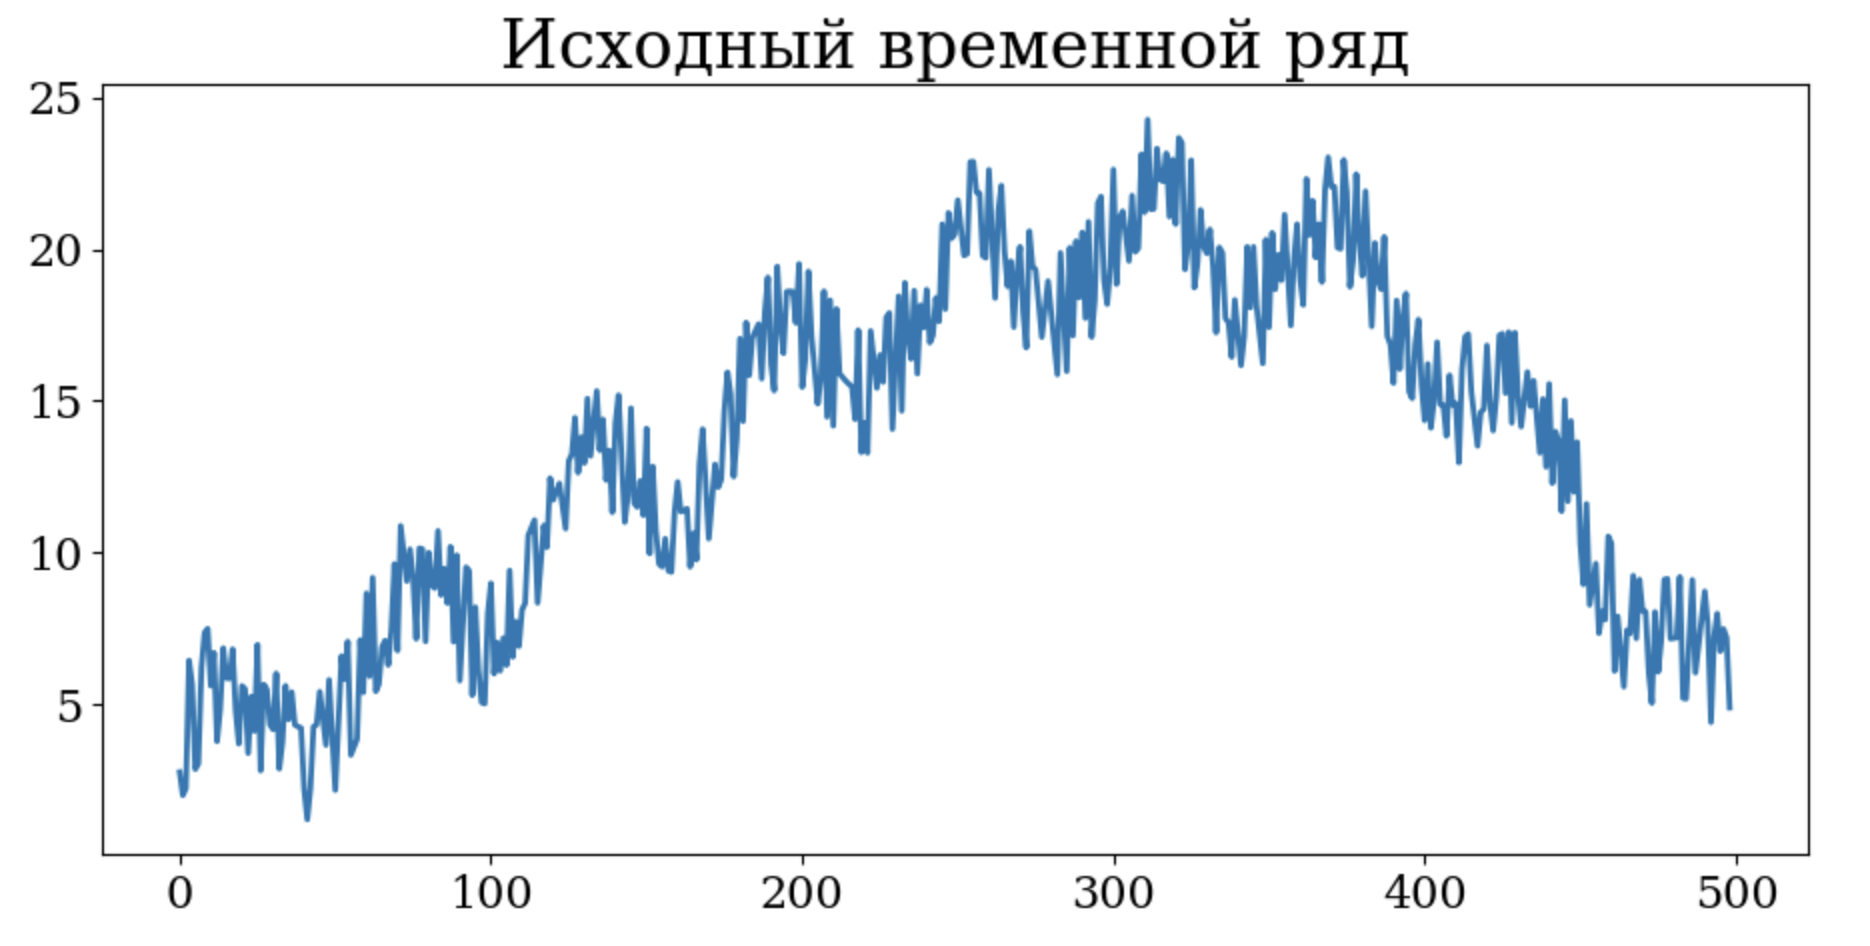
\includegraphics[width=0.45\linewidth]{lecture_3/fig/2_ts_init.png}
    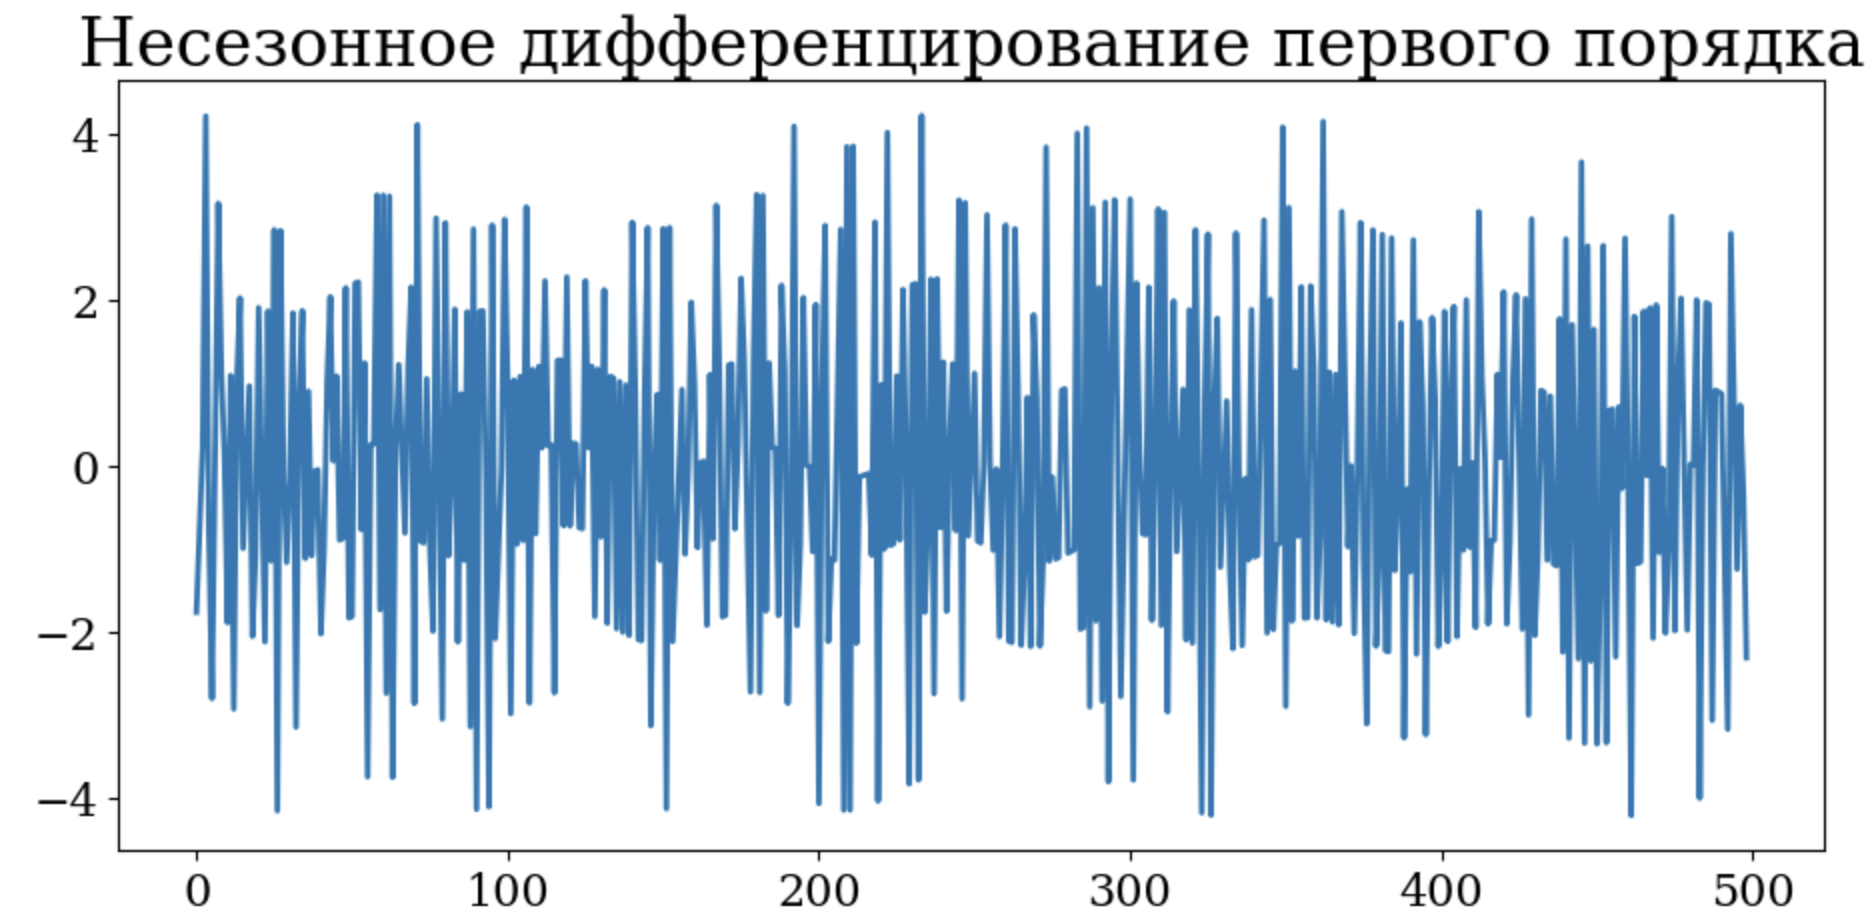
\includegraphics[width=0.45\linewidth]{lecture_3/fig/2_dts_init.png}
\end{figure}
\begin{figure}
    \centering
    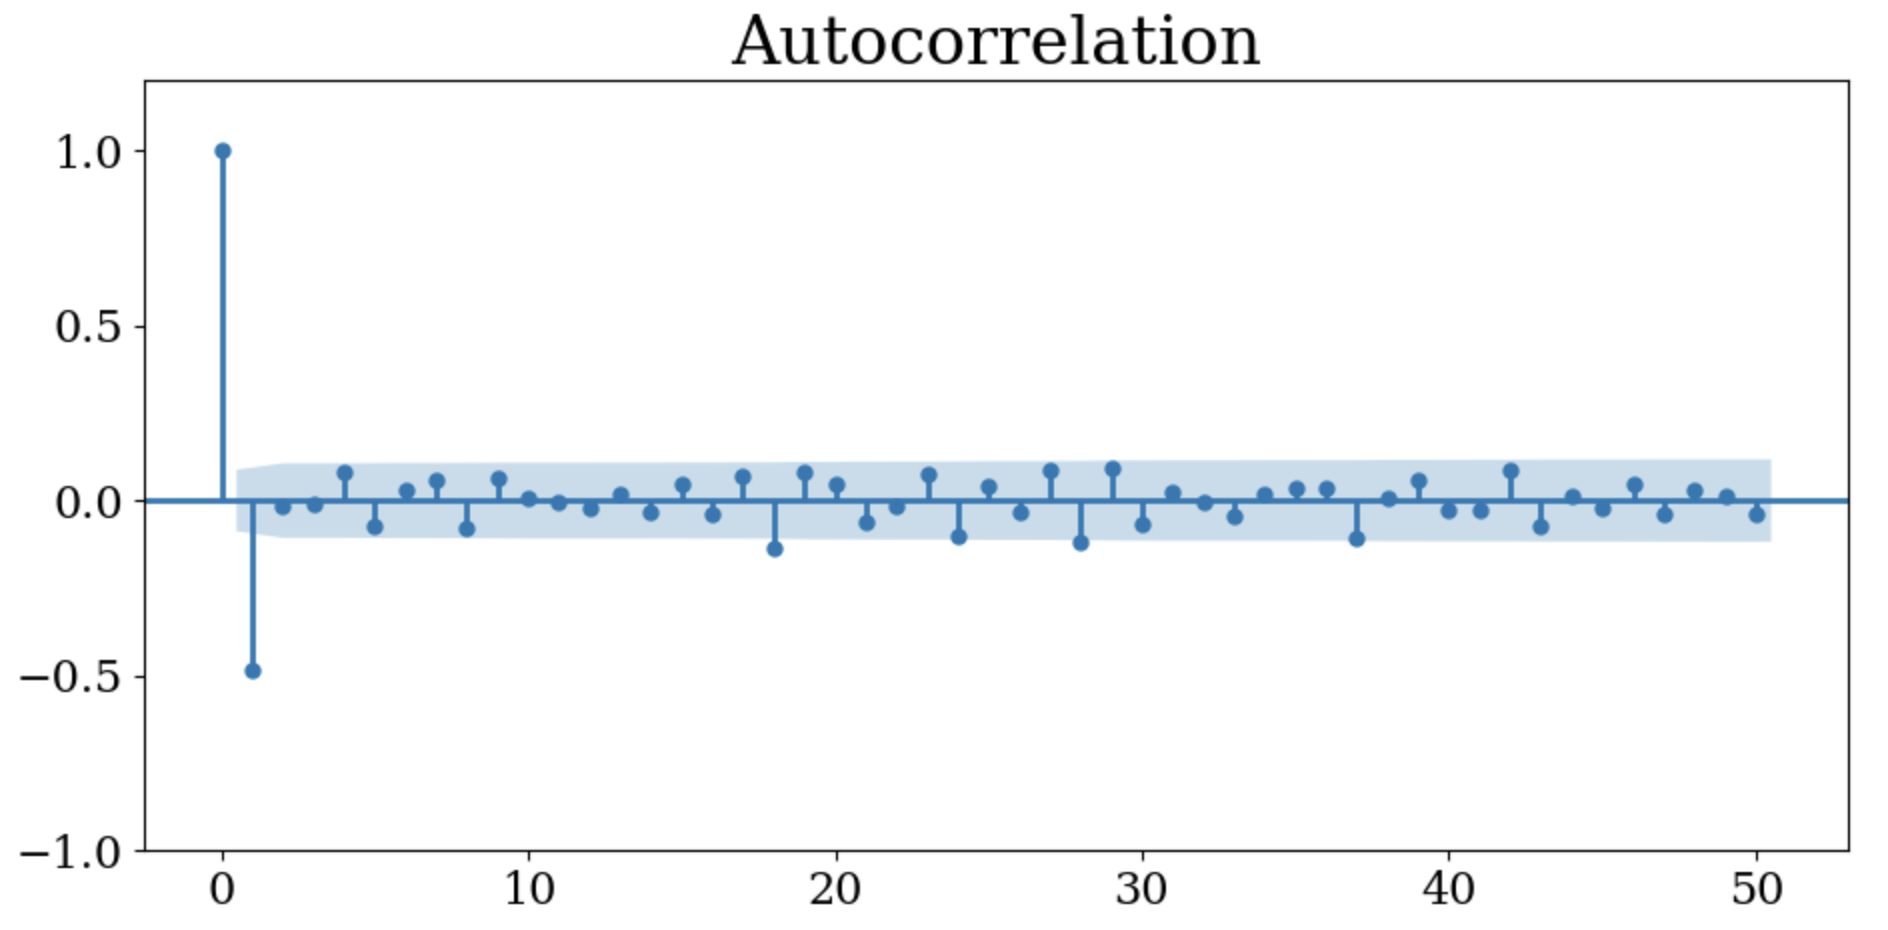
\includegraphics[width=0.45\linewidth]{lecture_3/fig/2_autocorr.png}
    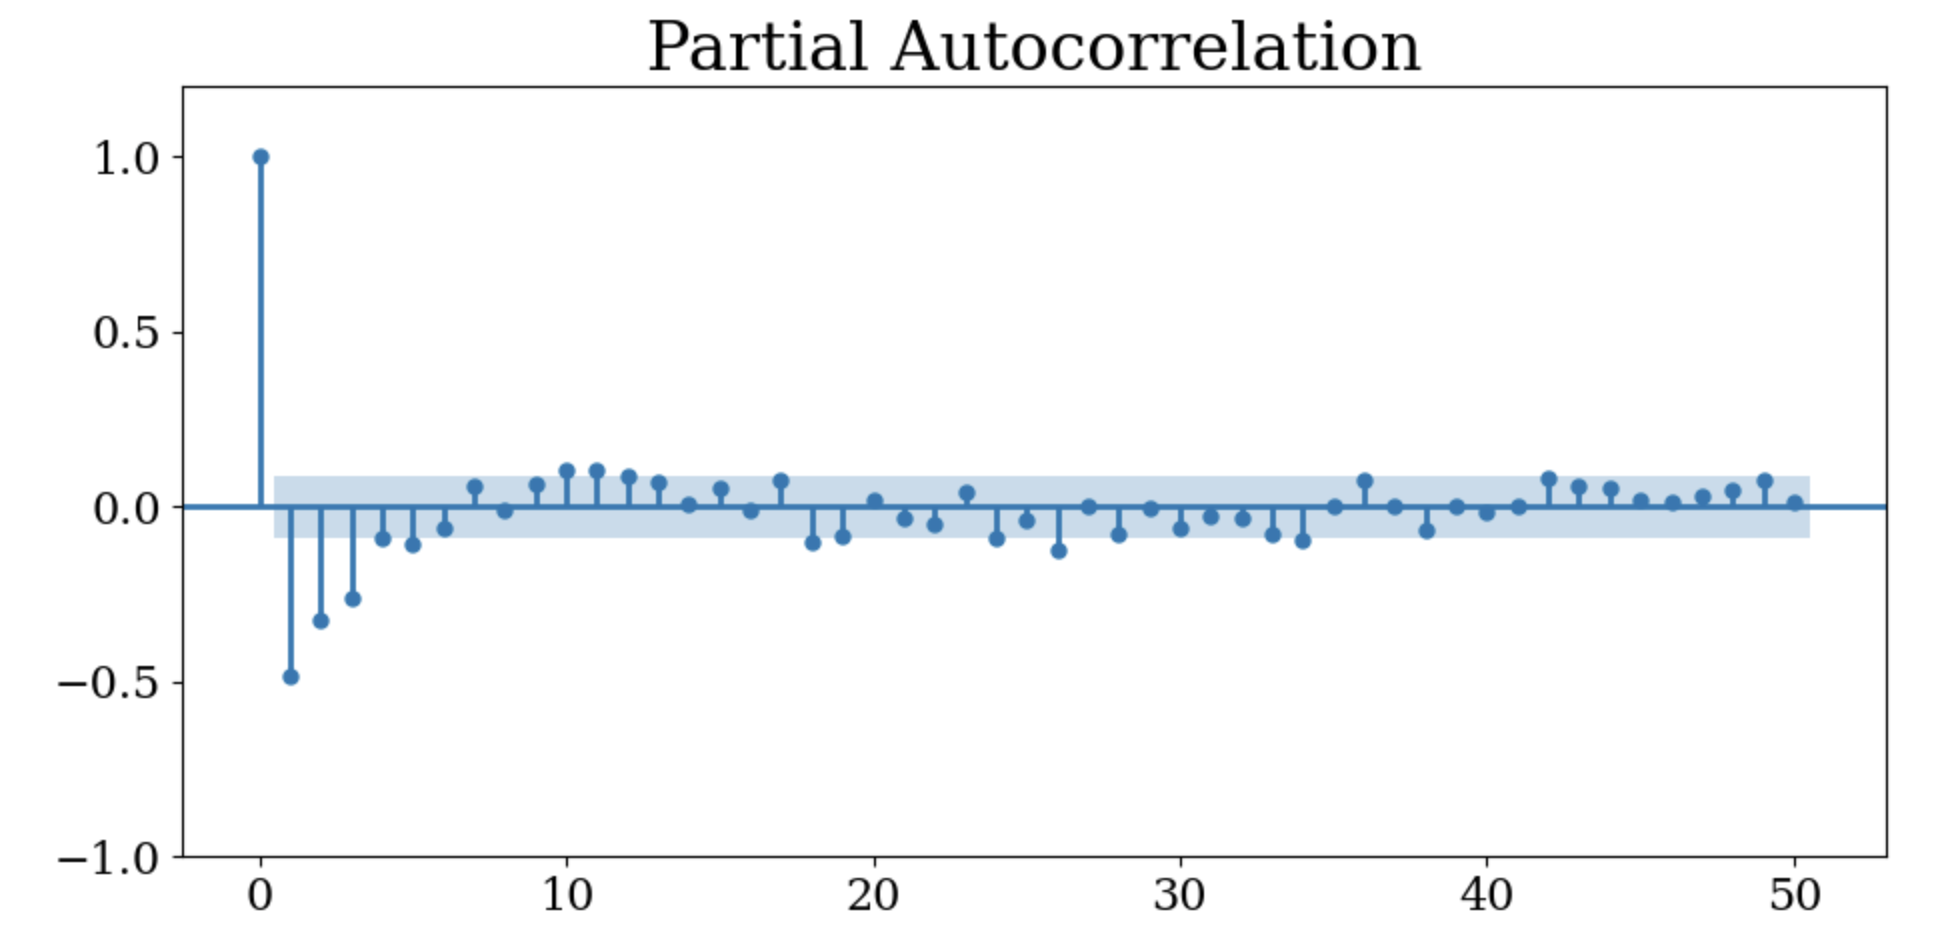
\includegraphics[width=0.45\linewidth]{lecture_3/fig/2_pautocorr.png}
\end{figure}

\begin{itemize}
    \item $Q*S$ --- номер последнего \textbf{сезонного} лага, при котором автокорреляция статистически значима;
    \item $q$ --- номер последнего \textbf{несезонного} лага,при котором автокорреляция статистически значима, меньше сезонного значения;
\end{itemize}

\end{frame}
%=======
\begin{frame}{Начальное приближение гиперпараметров}
\begin{figure}
    \centering
    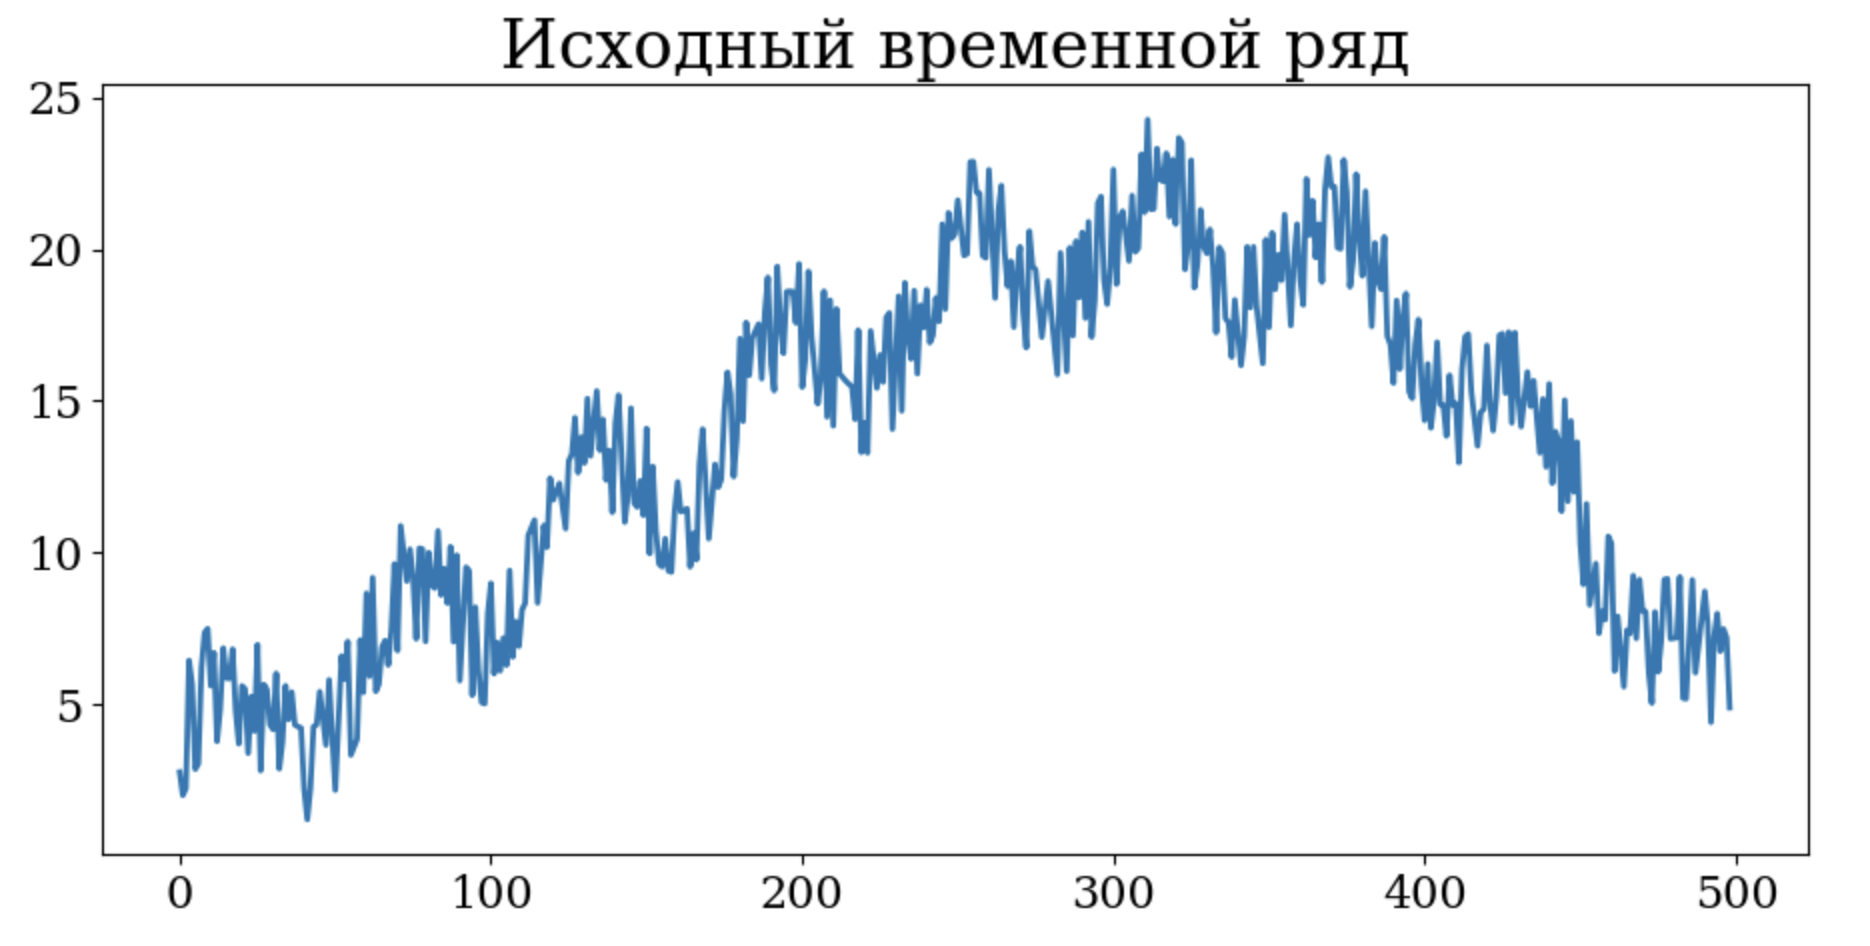
\includegraphics[width=0.45\linewidth]{lecture_3/fig/2_ts_init.png}
    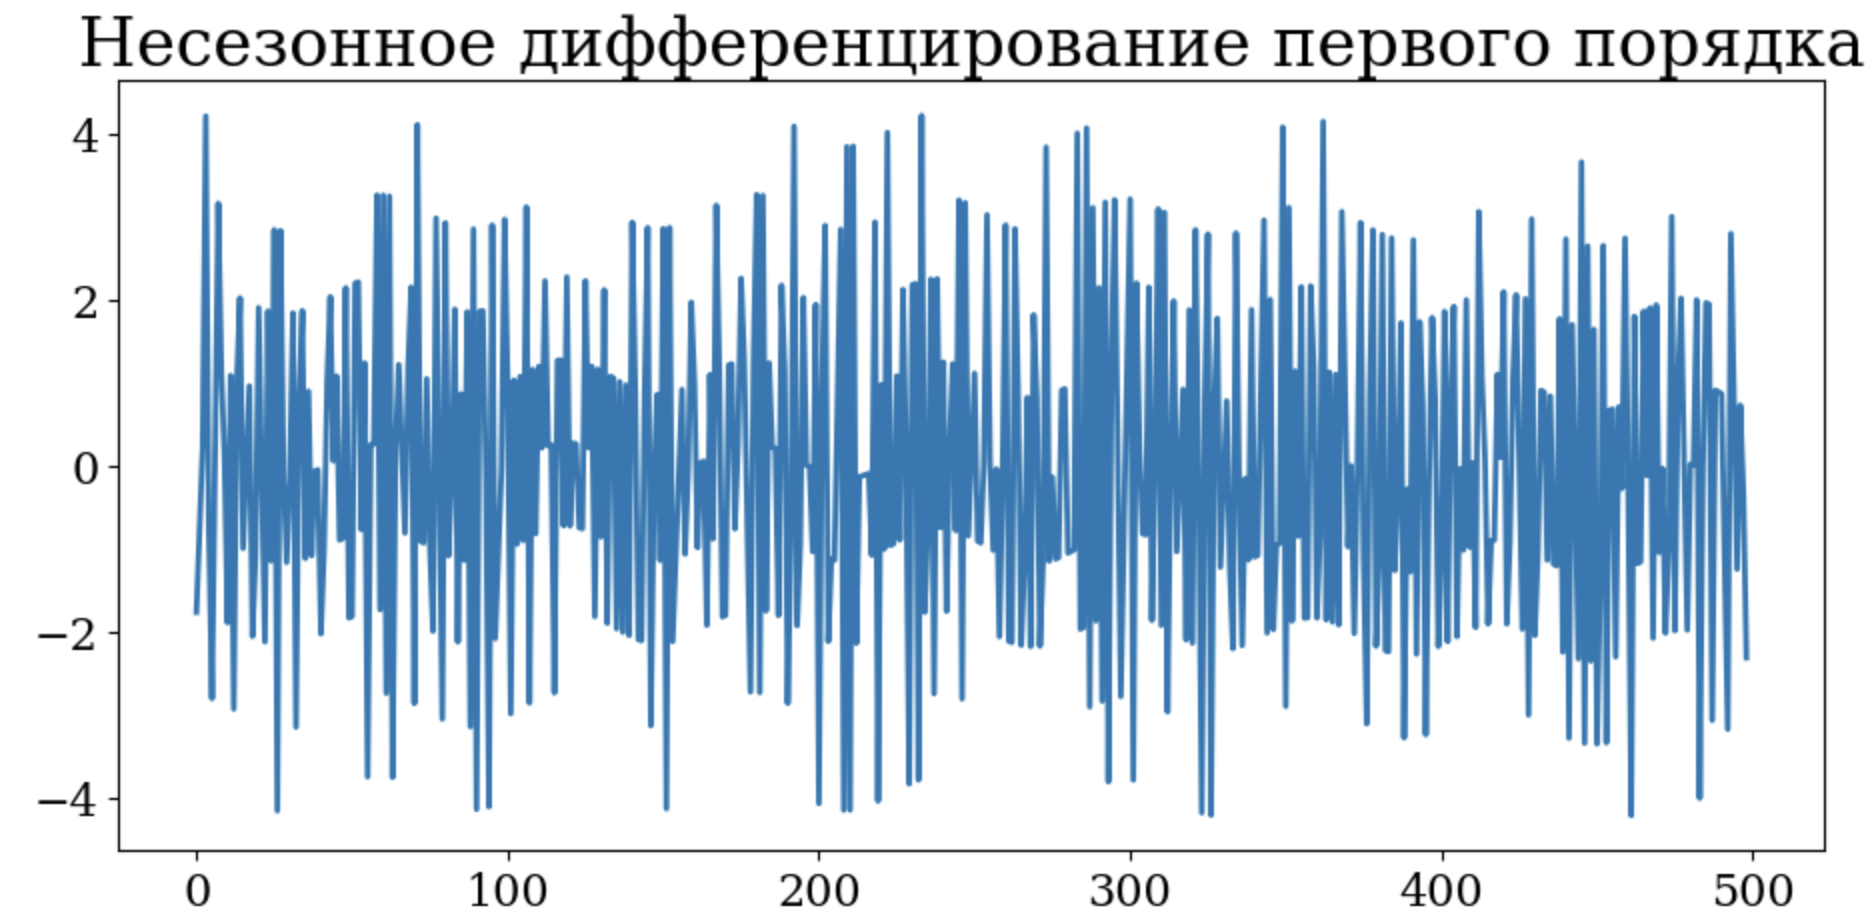
\includegraphics[width=0.45\linewidth]{lecture_3/fig/2_dts_init.png}
\end{figure}
\begin{figure}
    \centering
    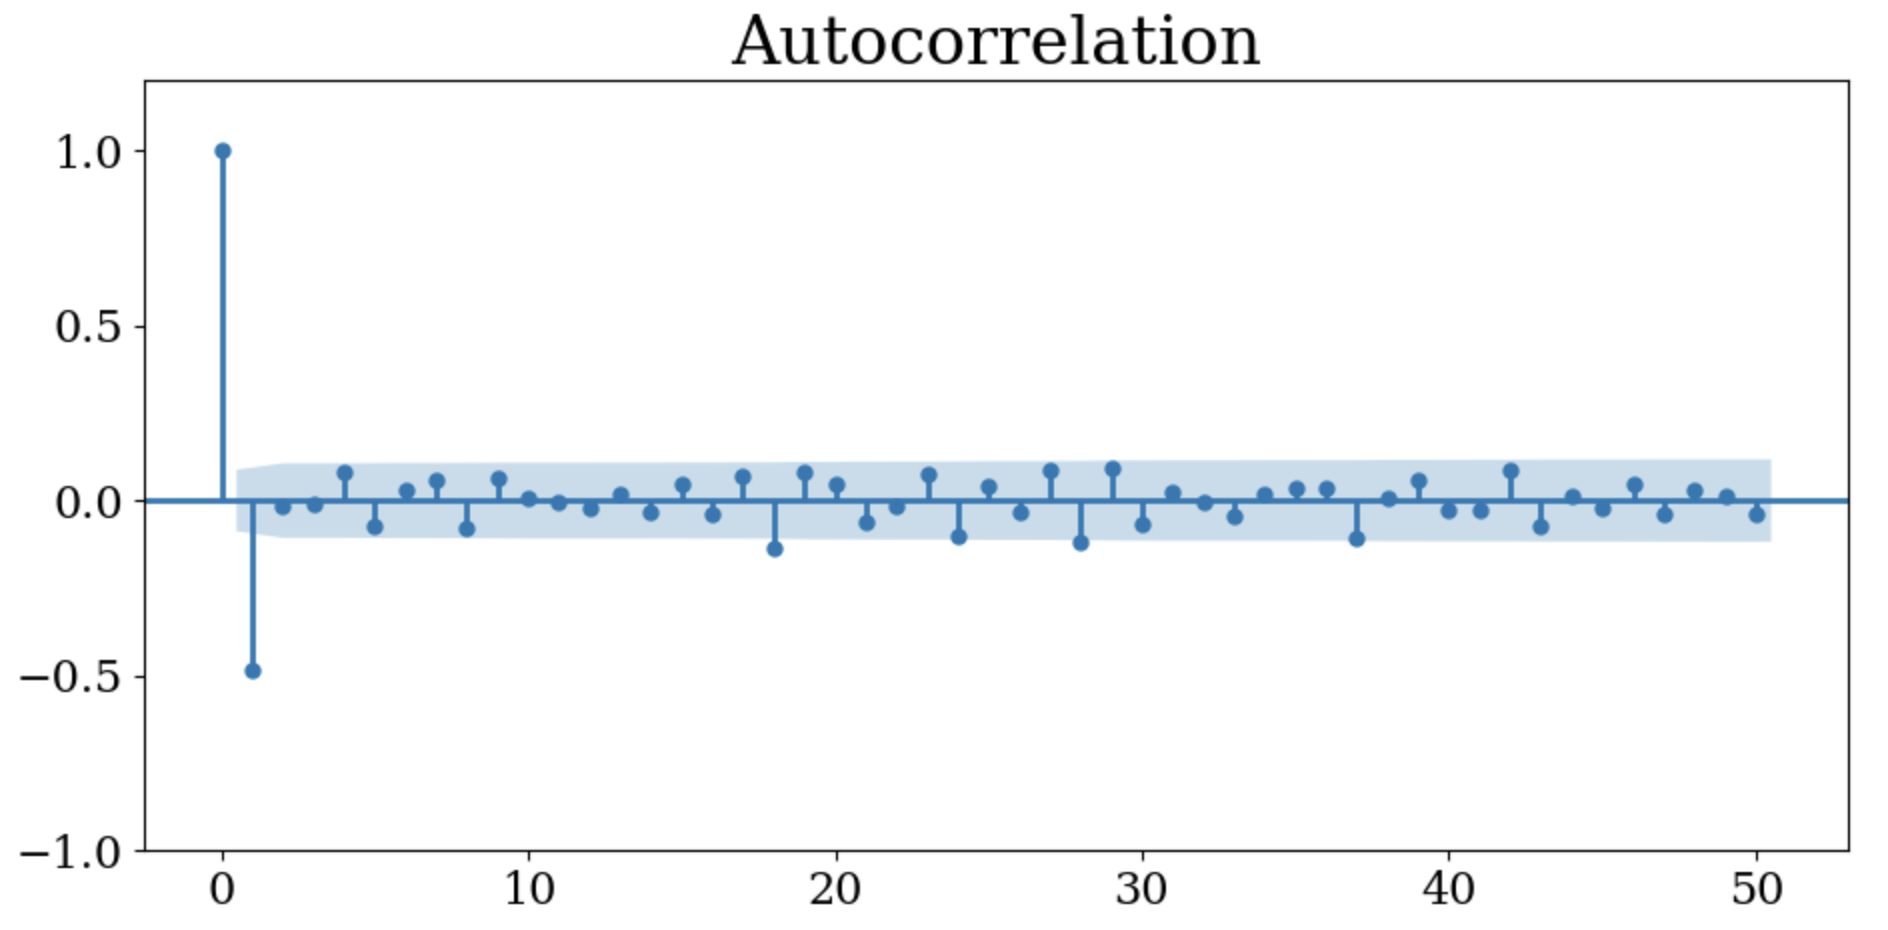
\includegraphics[width=0.45\linewidth]{lecture_3/fig/2_autocorr.png}
    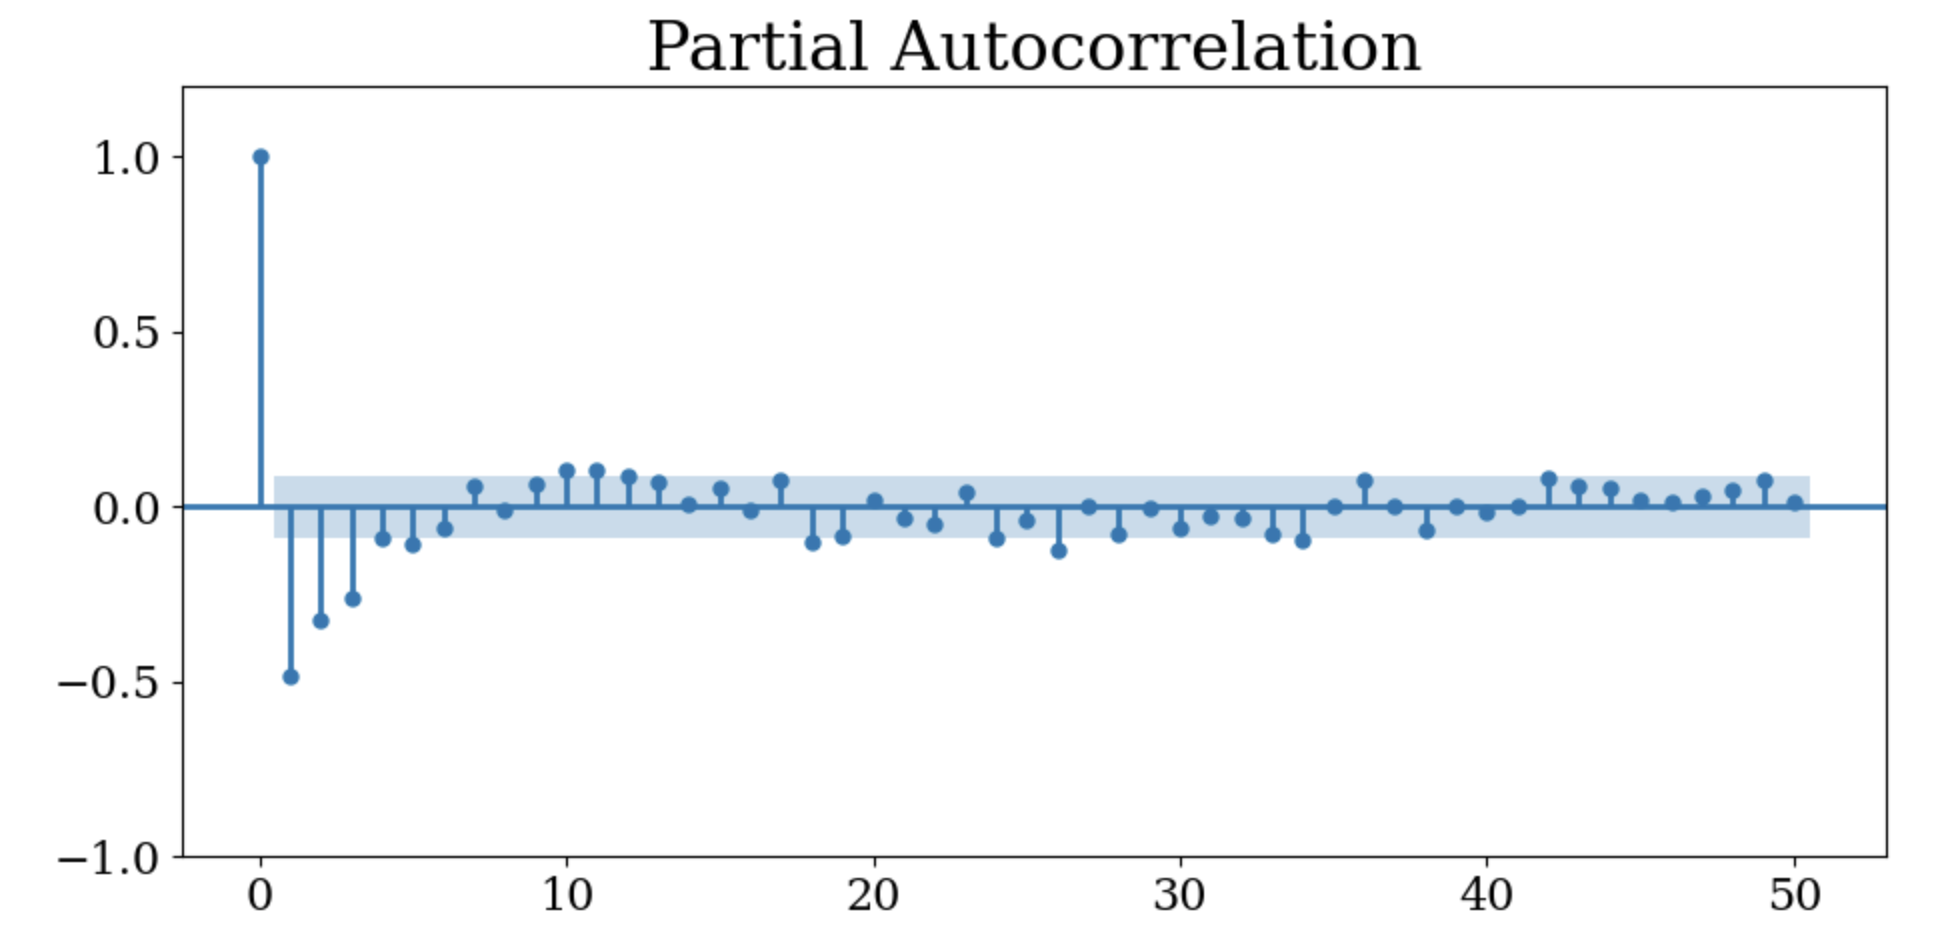
\includegraphics[width=0.45\linewidth]{lecture_3/fig/2_pautocorr.png}
\end{figure}

\begin{itemize}
    \item $P*S$ --- номер последнего \textbf{сезонного} лага, при котором \textbf{частичная} автокорреляция статистически значима;
    \item $p$ --- номер последнего \textbf{несезонного} лага,при котором \textbf{частичная} автокорреляция статистически значима, меньше сезонного значения;
\end{itemize}



\end{frame}
%=======
\begin{frame}{Проблема непостоянной дисперсии}
\begin{figure}
    \centering
    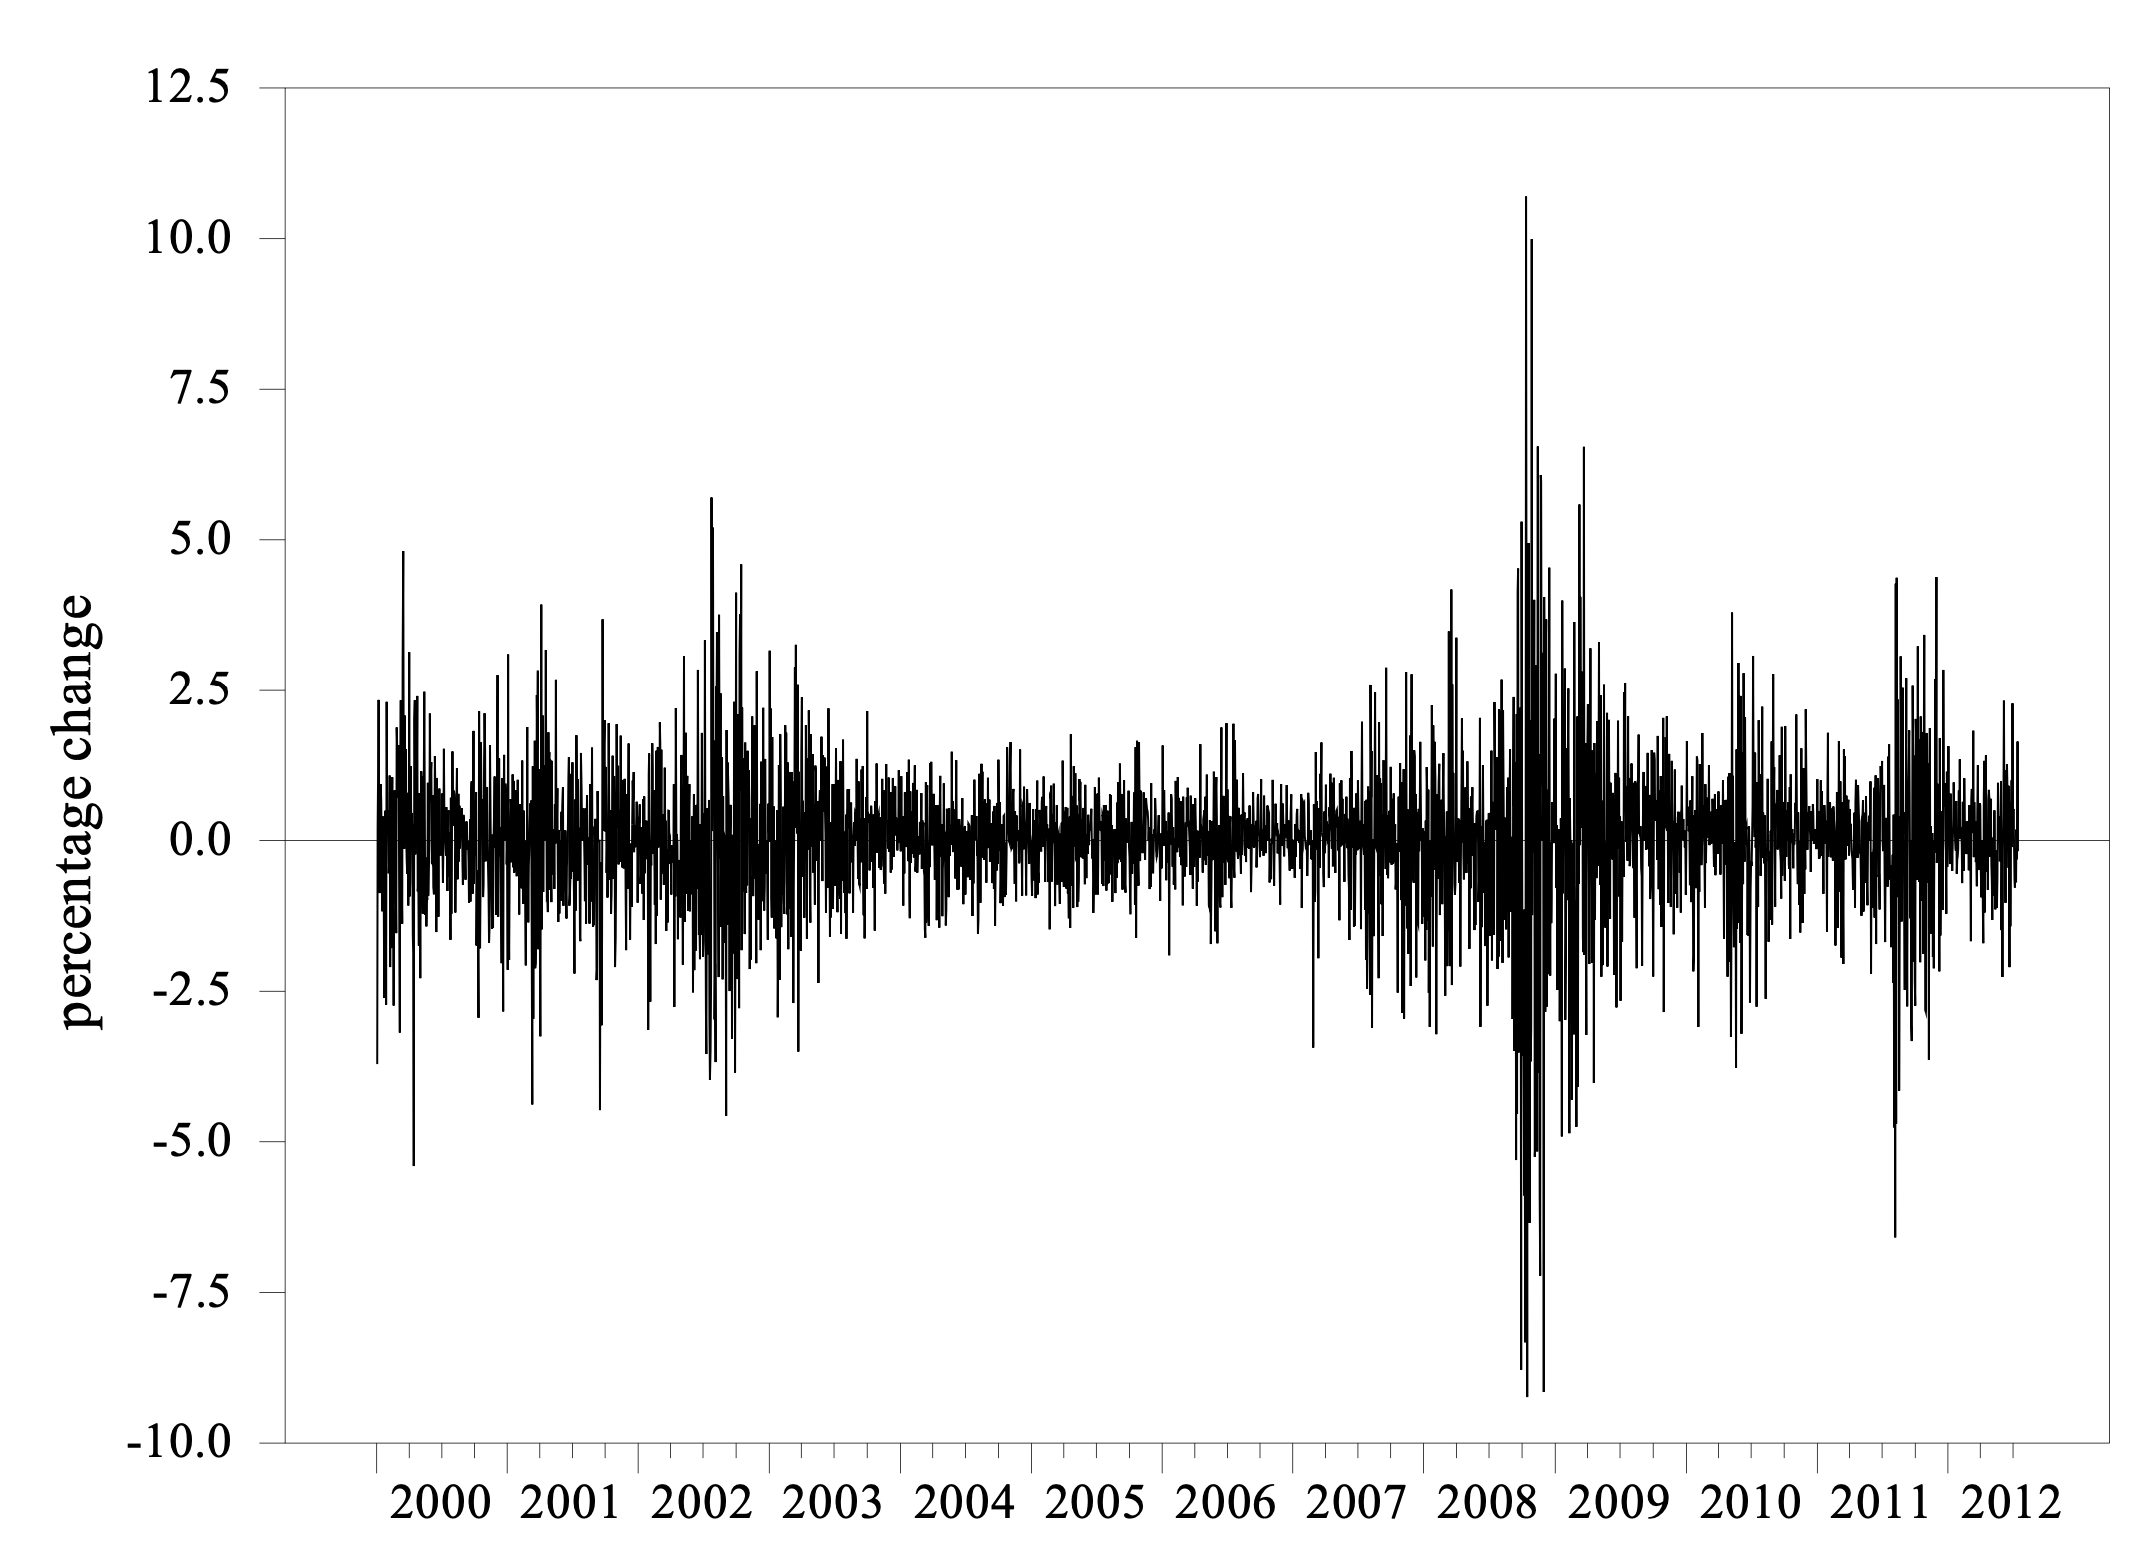
\includegraphics[width=0.9\linewidth]{lecture_3/fig/index_USA.png}
    \caption{Дневные изменения фондового индекса биржи}
\end{figure}
\end{frame}
%=======
\begin{frame}{ARCH и GARCH модели}
В традиционных эконометрических моделях дисперсия шума считается постоянной (гомоскедастичность).

Если временные ряды демонстрируют периоды необычно большой волатильности$^*$ , за которыми следуют периоды относительного спокойствия, предположение о постоянной дисперсии не выполняется. Для учета такого эффекта используются модели:
\begin{itemize}
    \item ARCH (autoregressive conditional heteroskedastic model),
    \item GARCH (generalized autoregressive conditional heteroskedastic
model).
\end{itemize}
\vspace{0.5cm}
$^*$ Термин \textbf{волатильность} в финансовой аналитике --- это отклонение доходности (непредсказуемая часть цен на активы).

\end{frame}


%=======
\begin{frame}{Изменяющаяся волатильность}
\begin{itemize}

\item Модель AR(1): $x_t = \mu + \phi_1 x_{t-1} + u_t = \mu_t + u_t$
\item Здесь $\mu_t$ и $u_t$ — ожидаемая часть с учетом истории и случайная часть соответственно.

\item Если ранее полагалось, что $u_t \sim WN(0,1)$, то теперь возмущения будут моделироваться с меняющейся во времени дисперсией $\sigma_t^2$: $$u_t =  z_t \sqrt{\sigma_t^2},$$ где $z_t \sim WN(0,1)$
\item $\sigma_t^2$ является функцией предыдущих значений ошибки $u_{t-1}, \ u_{t-2}, ...$.

\end{itemize}
\end{frame}
%=======
\begin{frame}{Историческая волатильность}
\textbf{Скользящее среднее}.
\begin{itemize}
    \item $$ \sigma_t^2 = \sum_{i=1}^{N}\frac{r_{t-i}^2}{N},$$
     где $r_t$ --- ошибка прошлых прогнозов,
    \item yчитывает изменения с задержкой,
    \item cложности с большим горизонтом прогнозирования.
\end{itemize}
\textbf{Экспоненциальное сглаживание}
\begin{itemize}
    \item $$ \sigma_t^2 = \lambda r_{t-1}^2 + (1-\lambda) r_{t-2}^2,$$
\item новый гиперпараметр $\lambda$,
\item нестабильный переход от \textquote{большой} дисперсии к \textquote{малой},
\item cложности с большим горизонтом прогнозирования.
\end{itemize}
\end{frame}
%=======
\begin{frame}{ARCH}
\begin{itemize}
\item  Одна из простых стратегий --- смоделировать меняющуюся дисперсию как процесс AR(q), используя квадраты оцененных остатков.
\item ARCH($p$): $ \sigma_t^2 = \alpha_0 + \alpha_1 u_{t-1}^2 + \alpha_2 u_{t-2}^2 + \dots + \alpha_p u_{t-p}^2 $,\\
где $\omega > 0, \ \alpha_i \geq 0 \ \forall i = \overline{1, p}$.
\item В отличие от скользящего среднего, здесь веса не обязательно равны 1/N.
\item Прогнозы: $ \mathrm{E}[u_{t+1}^2] = \sigma_{t+1}^2 = \alpha_0 + \alpha_1 u_{t}^2 + \alpha_2 u_{t-1}^2 + \dots + \alpha_p u_{t+1-p}^2 $.
\end{itemize}
\end{frame}
%=======
\begin{frame}{Примеры ARCH}
$$a)\quad z_t = WN(0,1),\quad b)\quad \quad u_t = z_t\sqrt{1 + 0.8u_{t-1}^2}$$
\begin{figure}
    \centering
    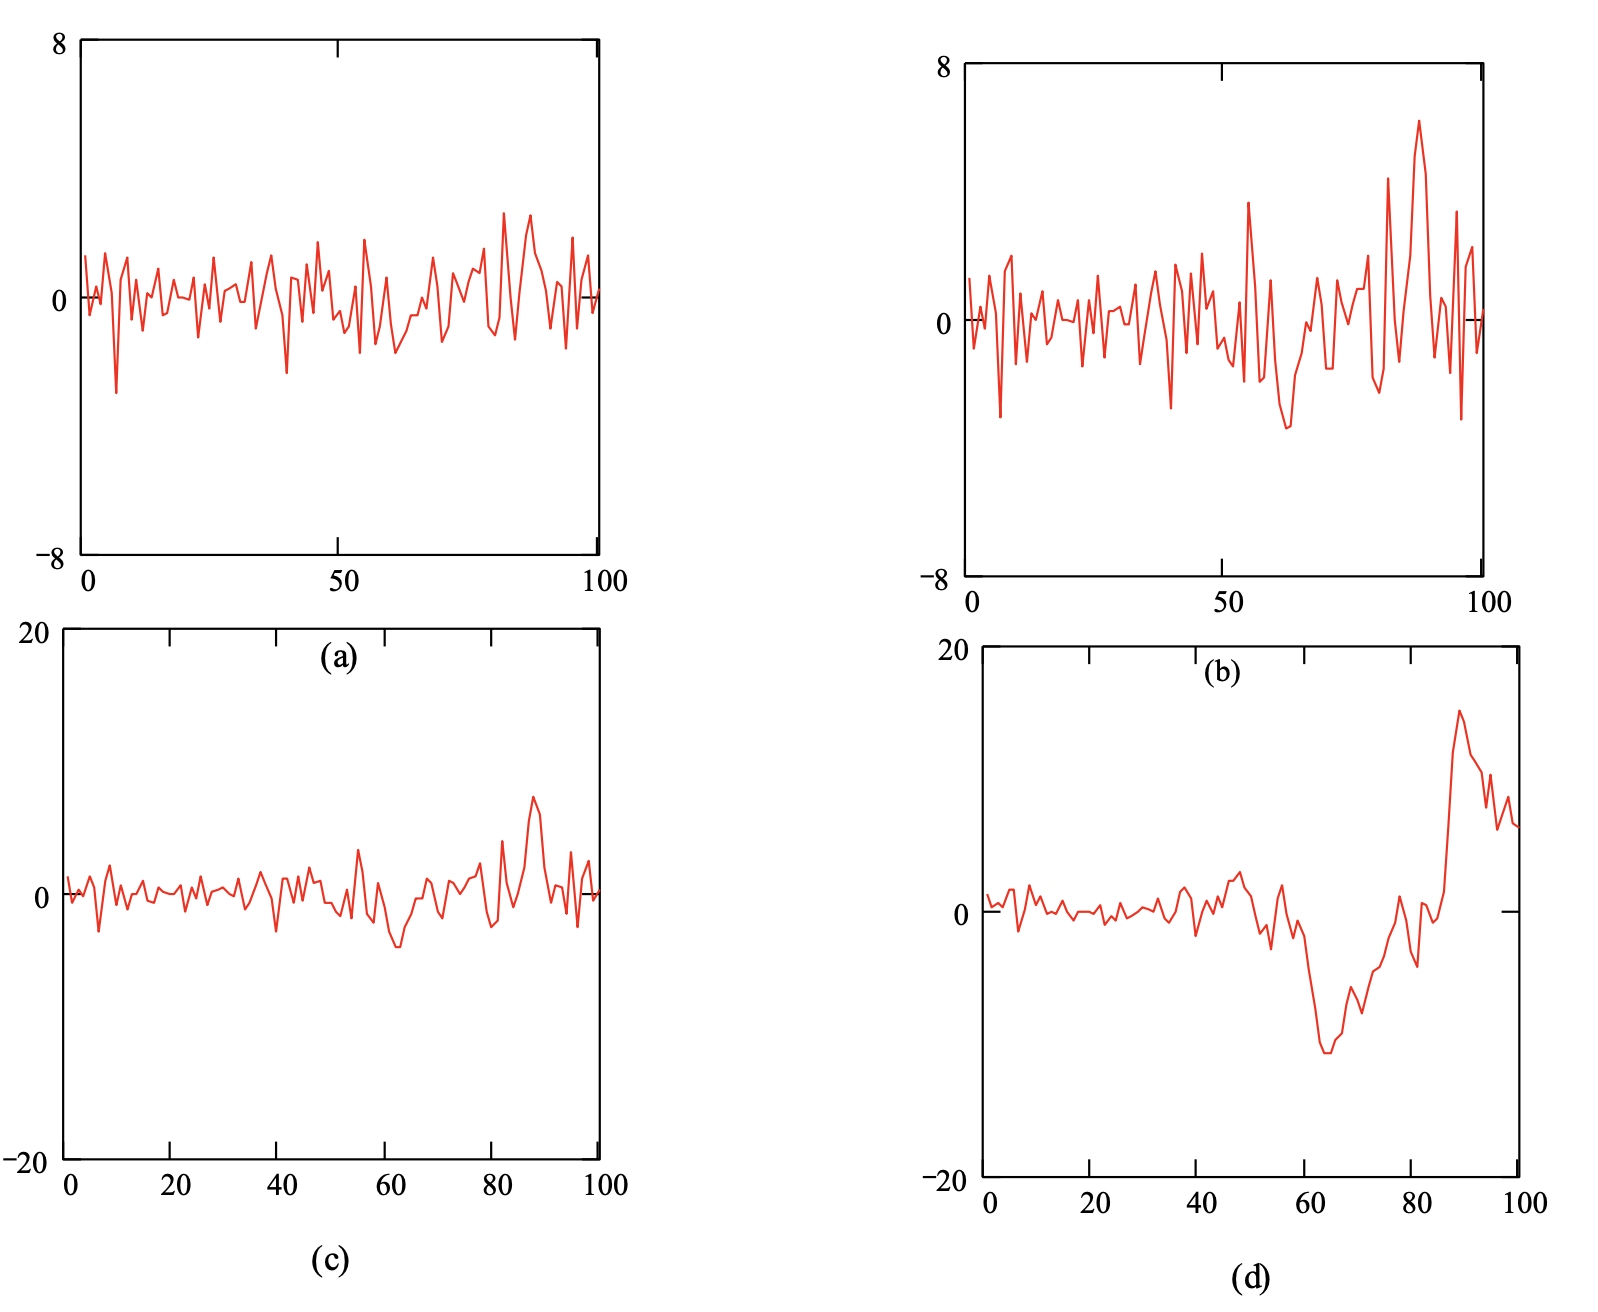
\includegraphics[width=0.7\linewidth]{lecture_3/fig/arch_example.png}
\end{figure}
$$c)\quad x_t = 0.2x_{t-1} + u_t,\quad \quad d)\quad x_t = 0.9x_{t-1} + u_t$$
\end{frame}
%=======
\begin{frame}{GARCH}
ARCH-модель предполагает зависимость дисперсии только от квадратов прошлых значений временного ряда.\\
\vspace{0.3cm}
Обобщить данную модель можно, предположив, что дисперсия зависит также от прошлых значений самой дисперсии (аналог ARMA).\\
\vspace{0.3cm}
\textbf{GARCH}($p, q$):
$$ \sigma_t^2 = \omega + \sum_{i=1}^p \alpha_i u_{t-i}^2 + \sum_{j=1}^q \beta_j \sigma_{t-j}^2$$
Здесь $\omega > 0, \ \alpha_i \geq 0 \ \forall i = \overline{1, p}, \ \beta_j \geq 0 \ \forall j = \overline{1, q}$. 
\end{frame}
%=======
\begin{frame}{GARCH}
\textbf{Основное преимущество:}
\begin{itemize}
\item Процесс ARCH(p) требует большого количества лагов для определения структуры зависимости, обычно встречающейся в \textquote{сложных} временных рядах.
\item Для этого необходимо оценивать множество параметров.
\item Модель GARCH допускает более гибкую и экономную спецификацию.
\end{itemize}
\end{frame}
%=======
\begin{frame}{GARCH}
\textbf{Некоторые важные недостатки}:
\begin{itemize}
    \item В моделях GARCH положительные и отрицательные возмущения одинаково влияют на дисперсии. Однако на практике такое изменение влияет на динамику временного ряда по-разному.
    \item В предыдущих моделях автокорреляционная функция экспоненциально убывает, но прикладные задачи показывают, что квадратичное затухание встречается чаще: такое высокое постоянство может быть достигнуто только с помощью сильно параметризованных GARCH моделей.
\end{itemize}

\end{frame}

%=======
\begin{frame}{Краткое повторение. Модель SARIMAX}
К модели SARIMA(p,d,q)(P,D,Q) добавляюся \textit{экзогенные} переменные, значение которых формируется вне модели.
Экзогенные переменные являются в модели независимыми величинами.
\begin{equation*}
x_t = \mu + \sum_{j=1}^{p}\phi_j x_{t-j} + u_t + \sum_{s=1}^{q}\theta_s u_{t-s} +...+ \textcolor{red}{\sum_{i=1}^{r}\beta_i x^{\text{exog}}_i}
\end{equation*}

\end{frame}
%=======
\begin{frame}{Модель векторной авторегрессии}
    \begin{itemize}
    \item Динамика сложных явлений описывается несколькими временными рядами.
    \item Временные ряды изменяются синхронно в определенной взаимозависимости.
    \item Необходимы методы совместного моделирования двух или более временных рядов.
    \end{itemize}
\end{frame}
%=======
\begin{frame}{Vector Autoregression (VAR)}
Рассмотрим подходы к методам совместного моделирования двух или более временных рядов. \\
\vspace{0.2cm}
Модель векторной авторегрессии VAR($p$) порядка $p$:
$$ x_t = \mu_1 + \sum_{j=1}^p \beta_j x_{t-j} + \sum_{j=1}^p \gamma_j y_{t-j} + u_t$$
$$ y_t = \mu_2 + \sum_{j=1}^p \delta_j x_{t-j} + \sum_{j=1}^p \theta_j y_{t-j} + v_t$$

Здесь $\beta, \gamma, \delta, \theta$ и $\mu$ - настраиваемые параметры модели, $u_t, v_t \sim WN(0,1)$.

\vspace{0.5cm}

\textbf{Важно}: в модели VAR все факторы рассматриваются как эндогенные.
\end{frame}
%=======
\begin{frame}{Vector Autoregression (VAR)}
В терминах матричных обозначений,
$$ \mathbf{x}_t = \boldsymbol{\mu} + \sum_{j=1}^p A_j \mathbf{x}_{t-j} + \mathbf{u}_t,$$
где $\mathbf{x}_t = 
\begin{pmatrix}
x_{1,t} \\
\vdots \\
x_{k,t}
\end{pmatrix}
$, 
$\boldsymbol{\mu} = 
\begin{pmatrix}
\mu_1 \\
\vdots \\
\mu_k
\end{pmatrix}
$, 
$\mathbf{u}_t = 
\begin{pmatrix}
u_{1,t} \\
\vdots \\
u_{k,t}
\end{pmatrix}
$, \\
\vspace{0.3cm}

$A_j$ -- матрицы размера $k \times k$.
\end{frame}
%=======
\begin{frame}{Vector Autoregression (VAR). Пример.}
\noindent
\begin{minipage}{0.4\textwidth}
    $$\text{VAR}: x_t = \mu_1 + A x_{t-j} + u_t $$

    \vspace{0.3cm}
    $$A = \begin{pmatrix}
            0.7 & 0.2 \\
            0.2 & 0.7
            \end{pmatrix}
    $$
    
    \vspace{0.3cm}
\end{minipage}
\hfill
\begin{minipage}{0.5\textwidth}\raggedleft
    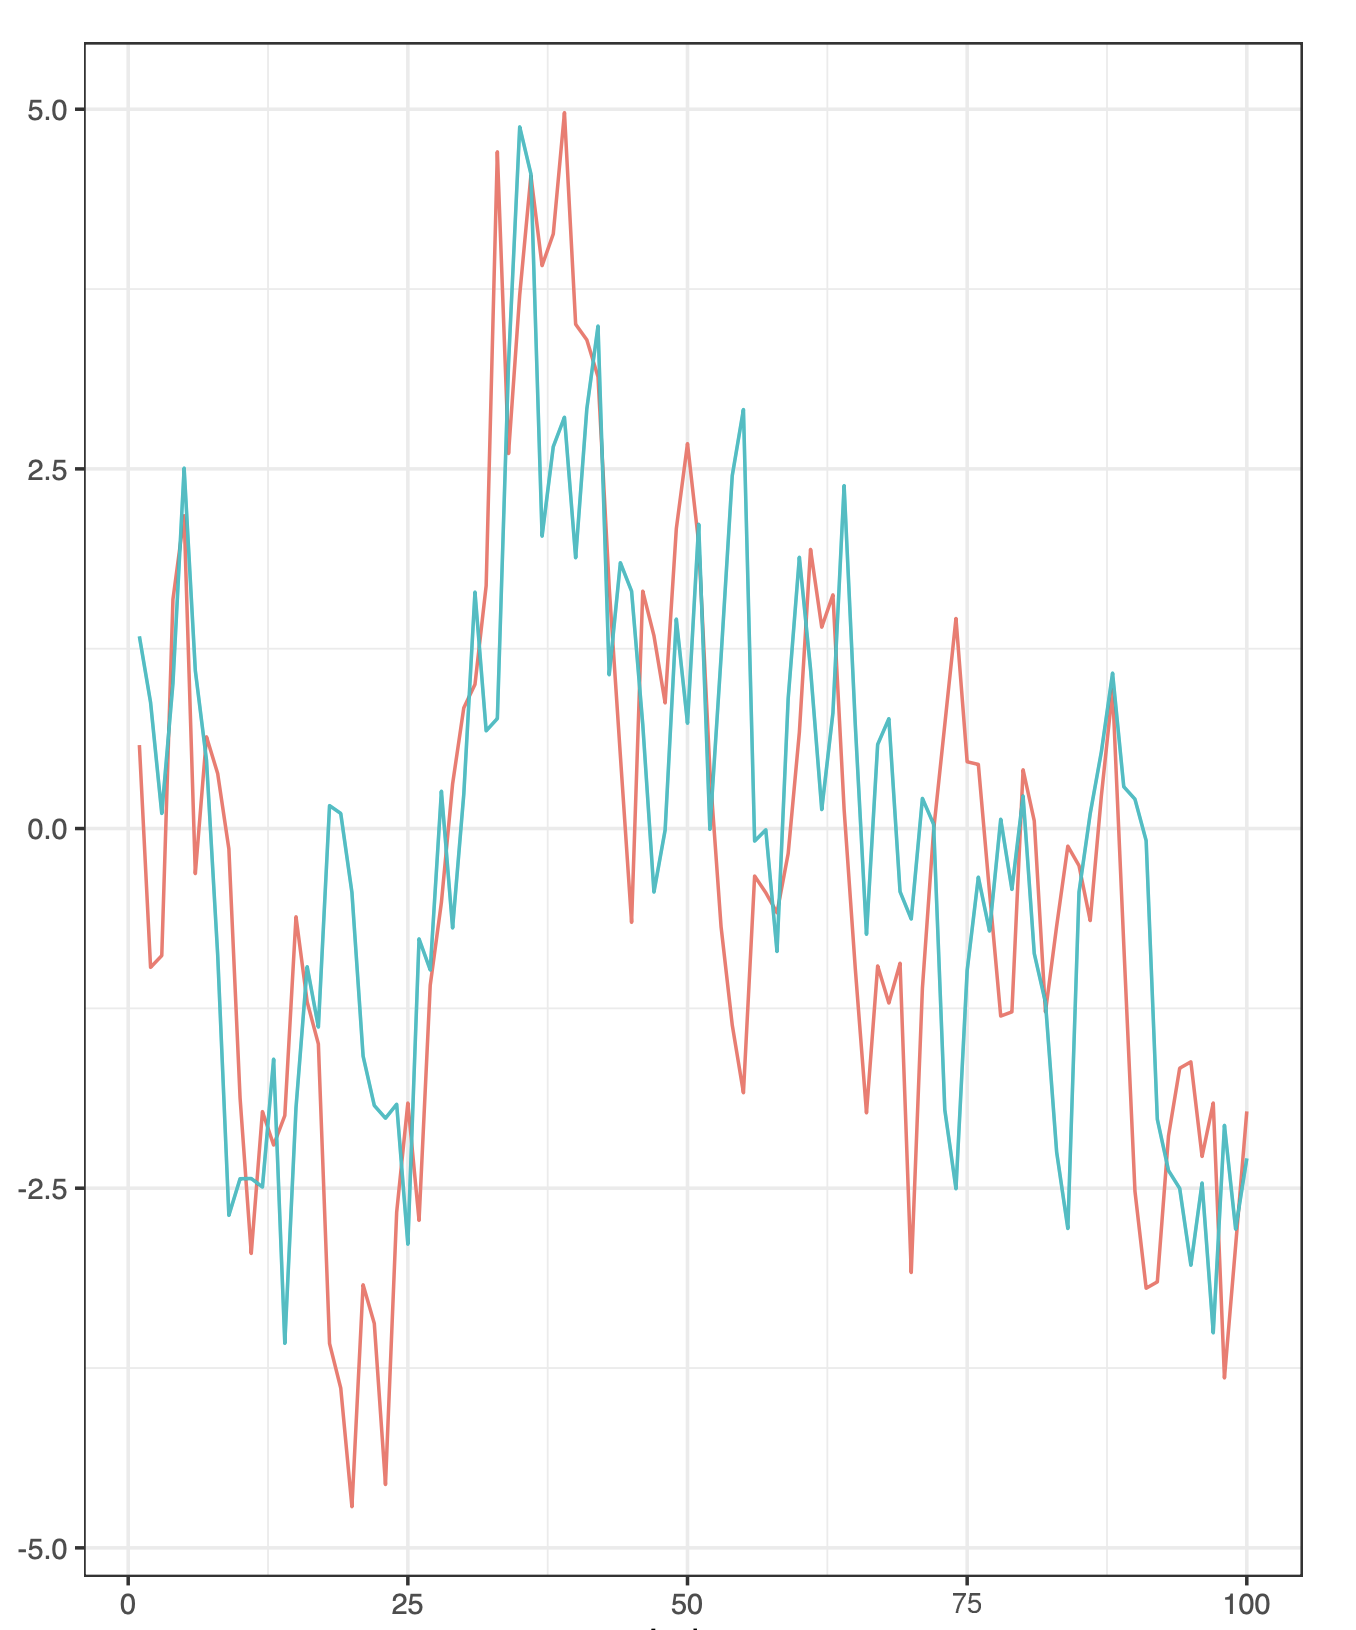
\includegraphics[width=0.9\linewidth]{lecture_3/fig/var_example.png}
\end{minipage}
%\vspace{0.2cm}
%\textbf{Важно}: коэффициенты VAR-модели в общем случае не интерпретируемы.
\end{frame}
%=======
\begin{frame}{Резюме}
\begin{itemize}
    \item При изменяющейся дисперсии ARMA не применима.
    \item Динамику изменения дисперсии описывает взвешенная сумма предыстории ошибок или оценок дисперсии.
    \item Модель AR, примененная к истории ошибок, приводит к модели ARCH.
    \item Модель GARCH --- это обобщение модели ARСH, использующее предысторию оценок диспресии $\sigma_t^2$.
    \item Созависимые временные ряды включаются в модель не только как экзогенные переменные.
    \item Многомерные временные ряды моделируются с помощью векторных моделей.
    \item Модель VAR --- векторная авторегрессия, моделирующая несколько временных рядов.
\end{itemize}
\end{frame}

\end{document} 